\chapter{State of the Art}
\label{chap:state-of-the-art}

\lettrine[lines=3, findent=3pt, nindent=0pt]{T}{his} chapter rounds out the theoretical background and technologies used in the project and discussed in the following: beginning with how network traffic is made ad how to characterize malicious activities, it will then be discussed Software Defined Networking as an industry standard and then \gls{ml} will be introduced, with particular emphasis on Intrusion Detection applications of \textit{Deep Learning}. The reader should here be provided with sufficient knowledge to understand chapters \ref{chap:methodology}, \ref{chap:results} and \ref{chap:conclusions}.

%----------------------------------------------------
% NETWORK TRAFFIC
%----------------------------------------------------

\section{Network Traffic}
\label{sec:network-traffic}

\textit{Network Traffic} is the amount of data that passes through a network at a given time, and it represents the starting point to the project. \\ Network architecture was thought to be modular and explicit, to ensure that modifications made to a single component were transparent to the rest of the system. This modularization is represented by \textit{network protocols} being separated into different layers: each layer has a precise task. In 1960s the \textit{U.S. Department of Defense} designed the \textit{TCP/IP} model, which is now the \textit{de facto} standard for protocols stack. Network security should be addressed at each TCP/IP network layer for different vulnerabilities and attack types \cite{Zaman2009}.

\begin{figure}[h!]
    \centering
    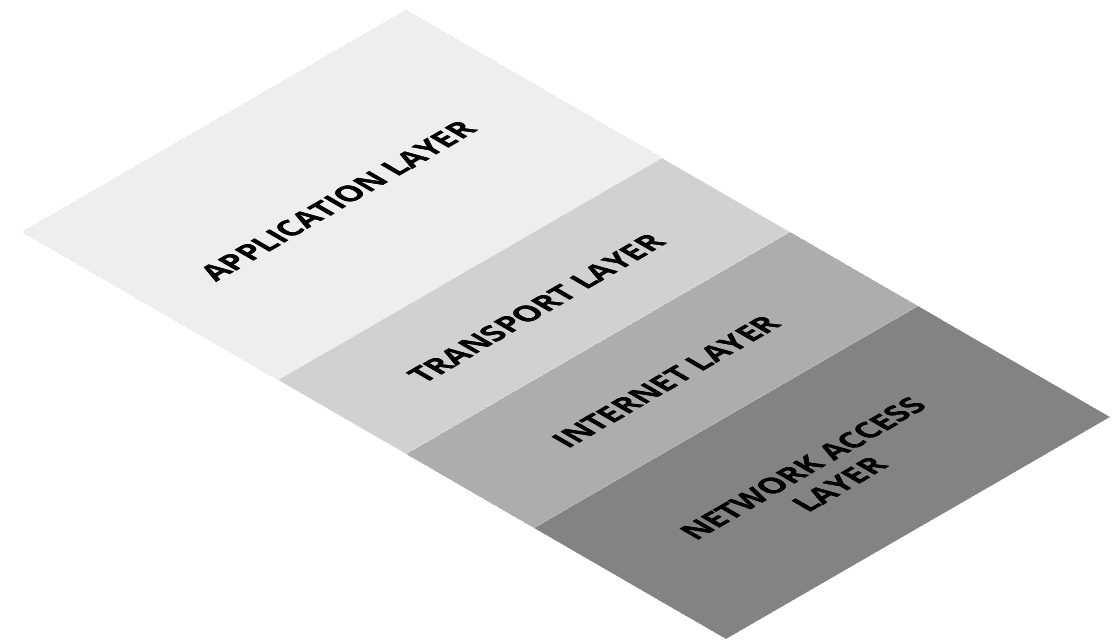
\includegraphics[scale=0.23]{figures/TCP_IP Stack.png}
    \caption{Internet protocol suite: TCP/IP Stack}
    \label{fig:TCP/IP-stack}
\end{figure}

TCP/IP stack is composed of 4 layers, representing from the physical connection (\textit{Network Access Layer}) to the user interface (\textit{Application Layer}). \\ The most relevant layer for this project is the third one: \textit{Transport Layer}, also called \textit{Host to Host Layer} is responsible for end-to-end communication and error-free delivery of data. It shields the upper-layer applications from the complexities of data. The main protocols used in this layer are:

\begin{itemize}
    \item[\faCaretRight] \gls{tcp}: provides reliable and error-free communication between end systems. It also has acknowledgement features and a flow control system. This protocol has a lot of overhead due to its features;
    \item[\faCaretRight] \gls{udp}: unlikely \glsxtrshort{tcp}, this protocol doesn't ensure a reliable connection between points, but it is very cost effective and lightweight.
\end{itemize}
Network packets are encapsulated in either a \textit{TCP segment} or a \textit{UDP datagram}. Another relevant protocol that will be used is \gls{icmp}, belonging to the second layer (\textit{Internet Layer}): it s responsible for providing hosts with information about network problems. Because of the particular design of network architecture, in which one layer acts as an intermediate between the layer above and the one below, when trying to characterize the traffic, looking only at these latter protocols can be sufficient \cite{Iglesias2015}.

%----------------------------------------------------
% MALICIOUS TRAFFIC
%----------------------------------------------------

\subsection{Malicious Network Traffic}
\label{subsec:malicious-traffic}

An \textit{intrusion} can be defined as an attempt to access information about computer systems or to damage system operation in an illegal or unauthorized manner \cite{Liu2019}, hence it will be considered \textit{malicious traffic} the entirety of network traffic generated by such operations. \\
The classes of malicious traffic analyzed in this work are the following:

\begin{itemize}
    \item[\faCaretRight] \textit{Botnet}: a botnet is a number of Internet connected devices, used to perform various tasks, from stealing data, to spam, or to practice \glsxtrshort{ddos} attacks. Automated infection tools can also be used to scan for and compromise suitable zombie systems \cite{icissp18} and \cite[p.~250]{Sharafaldin2019};
    \item[\faCaretRight] \textit{Bruteforce}: this kind of attack is one of the most popular and it can be used to guess passwords or \glsxtrshortpl{url} (in order to discover hidden contents in web applications). It can be defined as an hint and try attack, that corresponds of trying every possible key on a piece of ciphertext until an intelligible translation into plaintext is obtained \cite{icissp18} and \cite[p.~43]{Sharafaldin2019};
    \item[\faCaretRight] \gls{xss}: this kind of vulnerability can typically be found in web applications. An \glsxtrshort{xss} attack consist of injecting client-side scripts into \glsxtrshort{html} content of web pages, that can be viewed by other users and aims to gain elevated access privileges to sensitive data belong- ing to other sites \cite[p.~387]{Sharafaldin2019};
    \item[\faCaretRight] \gls{dos}: the objective of this attack is to exhaust some critical resources associated with the target service, denying or preventing legitimate users to access the system or the network \cite[p.~241]{Sharafaldin2019};
    \item[\faCaretRight] \gls{ddos}: unlike the previous type of attack, the incoming traffic flooding the victim is obtained from many different sources. This effectively makes it impossible to stop the attack simply by blocking a single source and guarantees much more bandwidth to the attacker \cite[p.~241]{Sharafaldin2019};
    \item[\faCaretRight] \textit{Heartbleed}: this particular attack exploits a bug in the OpenSSL cryptography library, widely used implementation of the \gls{tls} protocol. It was discovered in 2014 and allowed to expose significant amounts of memory on the vulnerable system \cite{Carvalho2014}, \cite{icissp18}, \cite{Stallings2014} and \cite[p.~706]{Sharafaldin2019};
    \item[\faCaretRight] \textit{Port Scanning}: this occurs when an attacker sends probe packets to gather intelligence information about the infrastructure, based on the responses received \cite{icissp18};
    \item[\faCaretRight] \gls{sqli}: it is one of the most prevalent and dangerous network-based security threats that uses malicious database queries to extract bulk data from the latter; this can occur, for example, through badly projected forms on web pages \cite[p.~163]{Sharafaldin2019}.
\end{itemize}
This list isn't exhaustive of all possible network violations, but these are the attacks contained in the dataset\footnote{See section \ref{subsec:datasets-for-evaluation}} used for the evaluation.

%----------------------------------------------------
% TRAFFIC CHARACTERIZATION
%----------------------------------------------------

\subsection{Traffic Characterization}
\label{subsec:traffic-characterization}

See paper \cite{Iglesias2015}, \cite{Sharafaldin2019} and  \cite{Velan2016} \\ Openflow \\
\lipsum[1]

\begin{table}[h]
    \centering
    \begin{tabularx}{0.8\textwidth}{p{3cm}Yp{2cm}}
        \toprule
        \textit{Attack} & \textit{Feature} & \normalfont\textit{Weight}\\
        \midrule
        \multirow{5}{*}{Botnet} & Flow Duration & 0.8\\
        \arrayrulecolor{gray75}\cmidrule{2-3}
        & Average Packet Size & A \\
        \cmidrule{2-3}
        & Something else & B \\
        \cmidrule{2-3}
        & Don't know & C \\
        \midrule
        \multirow{5}{*}{Bruteforce} & Total Length of Flow Packets & 0.8\\
        \cmidrule{2-3}
        & \glsxtrshort{ack} Flag Count & A \\
        \cmidrule{2-3}
        & \glsxtrshort{syn} Flag Count & B \\
        \cmidrule{2-3}
        & Don't know & C \\
        \midrule
        \multirow{5}{*}{DDoS} & Flow Duration & 0.8\\
        \cmidrule{2-3}
        & Average Packet Size & A \\
        \cmidrule{2-3}
        & Something else & B \\
        \cmidrule{2-3}
        & Don't know & C \\
        \midrule
        \multirow{5}{*}{Heartbleed} & Total Length of Flow Packets & 0.8\\
        \arrayrulecolor{gray75}\cmidrule{2-3}
        & Flow Duration & A \\
        \cmidrule{2-3}
        & Something else & B \\
        \cmidrule{2-3}
        & Don't know & C \\
        \midrule
        \multirow{4}{*}{Port Scan} & Init Win F.Bytes & 0.8\\
        \cmidrule{2-3}
        & B.Packets/s & A \\
        \cmidrule{2-3}
        & PSH Flag Count & B \\
        \arrayrulecolor{black}\bottomrule
    \end{tabularx}
    \caption{Useful network flow features}
    \label{tab:flow-metrics}
\end{table}

\lipsum[1-2]

%----------------------------------------------------
% SOFTWARE DEFINED NETWORKING
%----------------------------------------------------

\section{Software Defined Networking}
\label{sec:sdn}

\lipsum[1-3]

%----------------------------------------------------
% SOFTWARE DEFINED NETWORKING
%----------------------------------------------------

\subsection{SDN Controller}
\label{subsec:sdn-controller}

See paper \cite{Zhu2019} and \cite{Bondkovskii2016} \\
\lipsum[1-2]

%----------------------------------------------------
% INTRUSION DETECTION SYSTEMS
%----------------------------------------------------

\section{Intrusion Detection Systems}
\label{sec:intrusion-detection-system}

\lipsum[1-4]

    \begin{figure}[h!]
        \centering
        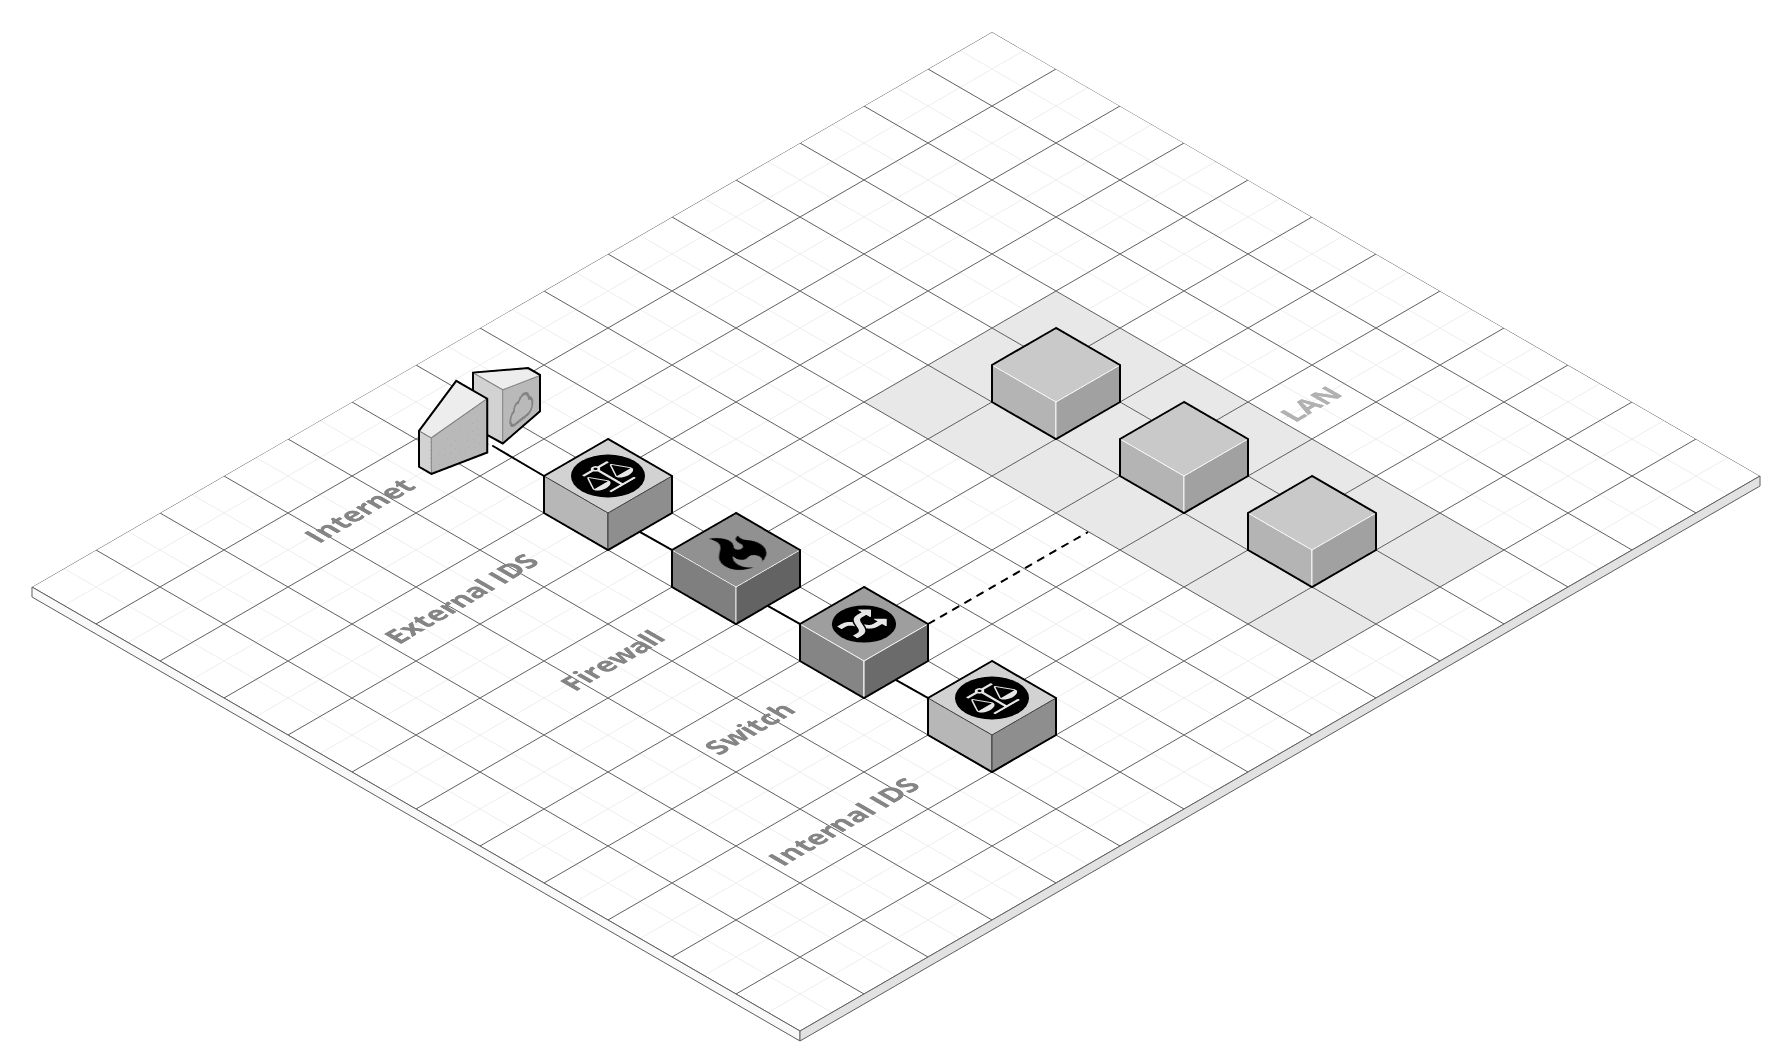
\includegraphics[scale=0.23]{figures/Intrusion Detection System Model.png}
        \caption{Intrusion Detection System Model}
        \label{fig:IDS-model}
    \end{figure}

%----------------------------------------------------
% DETECTION RATES
%----------------------------------------------------

\subsection{Detection rates}

See paper bla bla

%----------------------------------------------------
% TAXONOMY OF INTRUSION DETECTION SYSTEMS
%----------------------------------------------------

\subsection{Taxonomy of Intrusion Detection Systems}

See paper \cite{Liu2019}

%----------------------------------------------------
% DATASETS FOR INTRUSION DETECTION SYSTEMS
%----------------------------------------------------

\subsection{Datasets for Intrusion Detection Evaluation}
\label{subsec:datasets-for-evaluation}

See paper \cite{icissp18}, \cite{Khraisat2019} and \cite{Leevy2020} \\

\lipsum[1-6]

\begin{center}
    \begin{chronology}[5]{1983}{2010}{\textwidth}
        \event{1984}{One}
        \event[1985]{1986}{two}
        \event{\decimaldate{25}{12}{2001}}{three}
    \end{chronology}
\end{center}

%----------------------------------------------------
% MACHINE LEARNING
%----------------------------------------------------

\section{Machine Learning}
\label{sec:machine-learning}

See paper \cite{Khraisat2019} and \cite{Hodo2017} \\

\lipsum \\
Discussed in \ref{sec:machine-learning}

%----------------------------------------------------
% MACHINE LEARNING ALGORITHMS
%----------------------------------------------------

\subsection{Machine Learning Algorithms}
\label{subsec:ml-algorithms}

\lipsum

%----------------------------------------------------
% DEEP LEARNING
%----------------------------------------------------

\subsection{Deep Learning}
\label{subsec:deep-learning}

\lipsum

%----------------------------------------------------
% MACHINE LEARNING LIBRARIES
%----------------------------------------------------

\subsection{Machine Learning Libraries}
\label{subsec:ml-libraries}

\lipsum